%! suppress = Makeatletter
%! suppress = TooLargeSection
%! suppress = MissingLabel
\documentclass[12pt]{article}

% Fields
\usepackage{geometry}
\geometry{top=25mm}
\geometry{bottom=35mm}
\geometry{left=20mm}
\geometry{right=20mm}
% ------------------------------------------------

% Graphics
\usepackage{color}
\usepackage{tabularx}
\usepackage{tikz}
% https://tikz.dev/tikz-graphs
\usetikzlibrary{positioning, shapes.geometric, arrows, automata, graphs}
\tikzset{
    expr/.style={ellipse, draw=gray!60, fill=gray!5, very thick, minimum size=7mm, yshift=0.7cm},
    hexpr/.style={ellipse, draw=gray!60, fill=blue!15, very thick, minimum size=7mm, yshift=0.7cm},
    stmt/.style={rectangle, draw=gray!60, fill=gray!5, very thick, minimum size=5mm, yshift=0.7cm},
    decl/.style={rectangle, draw=blue!60, fill=gray!5, very thick, minimum size=5mm, yshift=0.7cm},
    hdecl/.style={rectangle, draw=blue!60, fill=blue!15, very thick, minimum size=5mm, yshift=0.7cm},
    subtree/.style={shape border rotate=90, isosceles triangle, draw=gray!60, fill=gray!5, very thick, minimum size=5mm, yshift=0.0cm},
}
\usepackage{blkarray}
\usepackage{graphicx}
\usepackage{forest} % https://tex.stackexchange.com/questions/198405/how-to-change-the-color-of-subtrees-in-tikz-qtree
% ------------------------------------------------

% Math
\usepackage{amsmath, amsfonts}
\usepackage{amssymb}
\usepackage{proof}
\usepackage{mathrsfs}
% Crossed-out symbols
% https://tex.stackexchange.com/questions/75525/how-to-write-crossed-out-math-in-latex
\usepackage[makeroom]{cancel}
\usepackage{mathtools}
% ------------------------------------------------

% Additional font sizes
% https://www.overleaf.com/learn/latex/Questions/How_do_I_adjust_the_font_size%3F
\usepackage{moresize}
% Additional colors
% https://www.overleaf.com/learn/latex/Using_colours_in_LaTeX
\usepackage{xcolor}
% \texttimes
\usepackage{textcomp}
% ------------------------------------------------

% Language
\usepackage[utf8] {inputenc}
\usepackage[T2A] {fontenc}
\usepackage[english, russian] {babel}
\usepackage{indentfirst, verbatim}
\usetikzlibrary{cd, babel}
% ------------------------------------------------

% Fonts
\usepackage{stmaryrd}
\usepackage{cmbright}
\usepackage{wasysym}
% ------------------------------------------------

% Code
% https://tex.stackexchange.com/questions/99475/how-to-invoke-latex-with-the-shell-escape-flag-in-texstudio-former-texmakerx
% Colored, requires --shell-escape compiling option
\usepackage{minted}
\setminted{xleftmargin=\parindent, autogobble, escapeinside=??}
\usepackage{listings}
% ------------------------------------------------

% Custom commands
\newcommand{\vocab}[1]{\textbf{#1}} % new word for vocabulary
\newcommand{\point}[1]{{\color{blue}\textit{#1}}} % point out something in text
\newcommand{\sembr}[1]{\llbracket{#1}\rrbracket} % semantic brackets
\newcommand{\positive}{$+$} % item: pros
\newcommand{\negative}{{\color{red} $-$}} % item: cons
\newcommand{\comb}[1]{\mathbf{#1}}
\newcommand{\step}{\rightsquigarrow}
\newcommand{\term}[1]{\mathbf{#1}}
\newcommand{\ap}{~}
\newcommand{\termdef}{\coloneqq}
\newcommand{\subst}[3]{\left[#2 \mapsto #3 \right] #1}
\newcommand{\eqbeta}{=_\beta}
\newcommand{\eqeta}{=_\eta}
% ------------------------------------------------

% Head
%\usepackage{fancybox,fancyhdr} not compatible with minted
\usepackage{hyperref}
%\pagestyle{fancy}
% ------------------------------------------------

% Bibliography
\usepackage{csquotes}
% https://tex.stackexchange.com/questions/3802/how-to-get-doi-links-in-bibliography
\usepackage{natbib}
\bibliographystyle{unsrtnat}
%\bibliographystyle{apalike}
%\bibliography{bib}
%\usepackage[backend=bibtex]{biblatex}
%\addbibresource{bib.bib}
%\addbibresource{bib}
% ------------------------------------------------

% Line numbers
% https://tex.stackexchange.com/questions/16010/number-every-line-of-pages
\usepackage{lineno}
\linenumbers
% ------------------------------------------------

% Enumerations
% https://tex.stackexchange.com/questions/10684/vertical-space-in-lists
\usepackage{enumitem}
\setlist{noitemsep} % nosep
% ------------------------------------------------

\begin{document}

    \begin{center}
    {\LARGE ФП 2.0}
        \\
        осень 2024
    \end{center}

    \tableofcontents

    \newpage

    \section*{Введение}

    В функциональном программировании и соответствующем языковом дизайне существует некоторый набор знаний, считающихся общеизвестным фольклором.
    Сложность в том, что эти знания рассеяны по книгам, статьям и ``культовым'' блог-постам, и требуется довольно много времени и сил для восстановления целостной картины.

    Цель этого курса --- собрать в одном месте такие фольклорные знания и организовать их в некоторую систему.
    Курс будет явным образом опираться на классические работы и помогать в их изучении.
    Просмотр упоминаемых статей является важной частью самостоятельной работы в рамках курсе.

    В связи с широтой контекста, этот курс является обзорным и не всегда глубоким.
    Так, детали реализации в GHC или теор-категорные основания вещей могут даваться в общем виде и без конкретики.
    В то же время в плоскости языкового дизайна через оптику функционального программирования и пользовательского опыта на Haskell курс пытается быть максимально подробным.

    Выбор тем и структура курса во многом обусловлены организацией языка Haskell, который этот курс использует как референсный.
    Не в последнюю очередь выбор тем для курса обусловлен интересами его автора.


    \section{Воспоминания о ФП}

    В этом разделе мы вспомним основные концепции функционального программирования и языка Haskell.

    \subsection{Термы и редукция}

    В ФП программы представляют собой выражения.
    Выполнение программ --- редукция таких выражений до более простых.
    Выражения можно представлять как в виде линейной записи символов, так и в виде дерева, для понимания которого не требуется знания вспомогательных правил ассоциативности и проч.

    Основная идея функционального программирования --- $\lambda$-абстракция.
    Она позволяет взять произвольное выражение и заменить его фрагмент на формальный параметр.
    Формальный параметр должен быть задекларирован выше по дереву с помощью специальной $\lambda$-вершины.
    Вместо формального параметра можно в дальнейшем подставлять различные конкретные параметры, то есть использовать одно выражение для различных целей.

    \begin{tikzpicture}
        \node [expr] (div) {$\div$};
        \node [expr] (x) [below left=of div] {$x$};
        \node [expr] (plus) [below right = of div] {$+$};
        \node [expr] (two) [below right = of plus] {$2$};
        \node [hexpr] (mult) [below left = of plus] {$\times$};
        \node [hexpr] (ten) [below left = of mult] {$10$};
        \node [hexpr] (four) [below right = of mult] {$4$};
        \draw[->] (plus) -- (div);
        \draw[->] (x) -- (div);
        \draw[->] (mult) -- (plus);
        \draw[->] (ten) -- (mult);
        \draw[->] (four) -- (mult);
        \draw[->] (two) -- (plus);
    \end{tikzpicture}
    \begin{tikzpicture}
        \node [hdecl] (f) {$f$};
        \node [hexpr] (lam) [below=of f] {$\lambda$};
        \node [hdecl] (y) [below right =of lam] {$y$};
        \node [expr] (div) [below=of lam] {$\div$};
        \node [expr] (x) [below left=of div] {$x$};
        \node [expr] (plus) [below right = of div] {$+$};
        \node [hexpr] (param) [below left=of plus] {$y$};
        \node [expr] (two) [below right = of plus] {$2$};
        \draw[->] (lam) -- (f);
        \draw[->] (div) -- (lam);
        \draw[->] (plus) -- (div);
        \draw[->] (x) -- (div);
        \draw[->] (two) -- (plus);
        \draw[->] (param) -- (plus);
        \draw[->] (y) -- (lam);
    \end{tikzpicture}
    \begin{tikzpicture}
        \node [hexpr] (app) {$@$};
        \node [hexpr] (f) [below left =of app] {$f$};
        \node [expr] (mult) [below right= of app] {$\times$};
        \node [expr] (ten) [below left= of mult] {$10$};
        \node [expr] (four) [below right= of mult] {$4$};
        \draw[->] (mult) -- (app);
        \draw[->] (f) -- (app);
        \draw[->] (ten) -- (mult);
        \draw[->] (four) -- (mult);
    \end{tikzpicture}

    Простейший функциональный язык --- $\lambda$-исчисление.
    Выражения в нём называются $\lambda$-термами.
    Термы можно сконструировать тремя способами:
    \begin{description}
        \item[Переменные] $x \in \Lambda$, если $x \in V$ \hspace{2em}
        \begin{tikzpicture}
            \node [expr] (x) {x};
        \end{tikzpicture}
        \item[Абстракция] $(\lambda x\ldotp M) \in \Lambda$, если $x \in V, M \in \Lambda$ \hspace{2em}
        \begin{tikzpicture}
            \node [expr] (lam) {$\lambda$};
            \node [decl] (x) [below right = of lam] {$x$};
            \node [subtree] (m) [below = of lam] {$M$};
            \draw[->] (m.north) -- (lam);
            \draw[->] (x) -- (lam);
        \end{tikzpicture}
        \item[Аппликация] $(M~N) \in \Lambda$, если $M \in \Lambda, N \in \Lambda$ \hspace{2em}
        \begin{tikzpicture}
            \node [expr] (dog) {$@$};
            \node [subtree] (m) [below left= of lam] {$M$};
            \node [subtree] (n) [below right= of lam] {$N$};
            \draw[->] (m.north) -- (lam);
            \draw[->] (n.north) -- (lam);
        \end{tikzpicture}
    \end{description}

    Редукция определяется следующим правилом переписывания: ищется применение $\lambda$-функции к аргументу и в её тело осуществляется подстановка аргумента во все свободные вхождения переменной, связанной лямбдой.

    \begin{tikzpicture}
        \node [expr] (top) {$\cdots$};
        \node [hexpr] (ap) [below = of top] {$@$};
        \node [hexpr] (lam) [below left = of ap] {$\lambda$};
        \node [decl] (x) [below right = of lam] {$x$};
        \node [subtree] (l) [below = of lam] {$M$};
        \node [subtree] (r) [below right = of ap] {$N$};
        \draw[->] (ap) -- (top);
        \draw[->] (lam) -- (ap);
        \draw[->] (l) -- (lam);
        \draw[->] (r.north) -- (ap);
        \draw[->] (x) -- (lam);
    \end{tikzpicture}
    \begin{tikzpicture}
        \node [expr] (top) {$\cdots$};
        \node [subtree] (bot) [below = of top] {$\subst{M}{x}{N}$};
        \draw[->] (bot) -- (top);
    \end{tikzpicture}

    \subsection{Типы}

    Программное обеспечение --- это сложно.
    Поэтому постоянно и неизбежно в программах возникают ошибки.
    Их можно искать, в том числе, статически, то есть без запуска программы.
    Одним из видов статического анализа является анализ типов.

    Как известно, выражение можно представить в виде дерева.
    Для примера рассмотрим $(\lambda y\ldotp x \div (y + 2)) \ap 3$:
    \\
    \begin{tikzpicture}
        \node [expr] (ap) {$@$};
        \node [expr] (three) [below right = of ap]{$3$};
        \node [hexpr] (lam) [below left =of ap] {$\lambda$};
        \node [hdecl] (y) [below right =of lam] {$y$};
        \node [expr] (div) [below=of lam] {$\div$};
        \node [expr] (x) [below left=of div] {$x$};
        \node [expr] (plus) [below right = of div] {$+$};
        \node [hexpr] (param) [below left=of plus] {$y$};
        \node [expr] (two) [below right = of plus] {$2$};
        \draw[->] (three) -- (ap);
        \draw[->] (lam) -- (ap);
        \draw[->] (div) -- (lam);
        \draw[->] (plus) -- (div);
        \draw[->] (x) -- (div);
        \draw[->] (two) -- (plus);
        \draw[->] (param) -- (plus);
        \draw[->] (y) -- (lam);
    \end{tikzpicture}

    Идея анализа типов состоит в том, что мы каждой вершине дерева программы пытаемся присвоить некоторую синтаксическую метку по определённым правилам.
    Если каждой вершине метку присвоить можно, то мы считаем, что программа проходит проверку типов, и она ``хорошая''.

    Пример выше проходит проверку типов в некоторой разумной системе типов:

    \begin{tikzpicture}
        \node [expr] (ap) {$@ : int$};
        \node [expr] (three) [below right = of ap]{$3 : int$};
        \node [hexpr] (lam) [below left=of ap] {$\lambda : int \to int$};
        \node [decl] (y) [below right = of lam] {$y {\color{red}~: int}$};
        \node [expr] (div) [below=of lam] {$\div : int$};
        \node [expr] (x) [below left=of div] {$x : int$};
        \node [expr] (plus) [below right = of div] {$+ : int$};
        \node [hexpr] (param) [below left=of plus] {$y : int$};
        \node [expr] (two) [below right = of plus] {$2 : int$};
        \draw[->] (lam) -- (ap);
        \draw[->] (three) -- (ap);
        \draw[->] (div) -- (lam);
        \draw[->] (plus) -- (div);
        \draw[->] (x) -- (div);
        \draw[->] (two) -- (plus);
        \draw[->] (param) -- (plus);
        \draw[->] (y) -- (lam);
    \end{tikzpicture}

    Система типов определяет синтаксис типовых меток и правила, по которым их можно приписывать.
    Синтаксис обычно описывается в классических нотациях а ля BNF, а правила в виде типовых дробей.
    Например, так выглядят дроби для просто-типизированного $\lambda$-исчисления:
    \[
        \begin{array}{l c r}
            \infer[ctx]{\Gamma \vdash x: \sigma}{(x: \sigma) \in \Gamma}
            &
            \infer[elim\to]{\Gamma \vdash M\;N : \tau}{\Gamma \vdash M : \sigma \to \tau & \Gamma \vdash N : \sigma}
            &
            \infer[intro\to]{\Gamma \vdash \lambda x^{\color{red} \sigma}\ldotp M : \sigma \to \tau}{\{x : \sigma\} \cup \Gamma \vdash M : \tau}
        \end{array}
    \]

    Типовые метки имеют чисто-синтаксическую природу, однако их можно проинтерпретировать.
    Самая популярная интерпретация~--- воспринимать типовую метку как множество.
    Так, метке $int \to int$ можно поставить в соответствие множество функций между множествами ограниченных целых чисел.

    \subsection{Функции в Haskell}

    В своей основе Haskell представляет собой расширенное типизированное $\lambda$-исчисление, дополненное примитивными типами, возможностью декларировать новые имена, структурами данных и классами типов.

    Примеры $\lambda$-абстракций в REPL окружении GHCi:

    \begin{minted}{haskell}
        ghci> (\x -> x + 1) 4
        5
    \end{minted}

    Можно узнать тип функции в интерпретаторе (в реальности числа полиморфные, но об этом далее):
    \begin{minted}{haskell}
        ghci> :t \x -> x + 1
        \x -> x + 1 :: Int -> Int
    \end{minted}

    Функциям можно давать имена.
    Именам можно приписывать типы, это рекомендуется делать явно для деклараций на верхнем уровне файлов исходного кода.
    \begin{minted}{haskell}
        f :: Int -> Int
        f x = x + 1
    \end{minted}

    Если имя типа начинается с маленькой буквы, то это не конкретный заранее заданный тип, а типовая переменная, способная принимать различные значения в зависимости от контекста.
    Такая возможность называется \point{параметрическим полиморфизмом}.
    Так, функция, которая просто возвращает свой аргумент, никак не ограничивает тип аргумента.
    Но в то же время тип результата должен совпадать с типом аргумента.
    \begin{minted}{haskell}
        id :: a -> a
        id x = x

        ghci> :t id 5
        id 5 :: Int
    \end{minted}

    Функции могут принимать другие функции в качестве аргументов.
    Имя функции может состоять из специальных символов, тогда она считается оператором и может применяться к своим операндам в инфиксном стиле:
    \begin{minted}{haskell}
        ($) :: (a -> b) -> a -> b
        f $ x = f x
    \end{minted}

    Пример рекурсивной функции, использующей охранные выражения для отличения базового случая рекурсии:
    \begin{minted}{haskell}
        factorial :: Int -> Int
        factorial n
          | n < 1 = 1
          | otherwise = n * factorial (n - 1)
    \end{minted}

    \subsection{Данные в Haskell}

    В Haskell есть встроенная возможность объявлять свои типы данных, а так же создавать их экземпляры.

    Зададим тип данных, описывающий животных:
    \begin{minted}{haskell}
        data Animal
          = Cat String Int
          | Dog String
    \end{minted}

    Мы задали тип данных \texttt{Animal} и два способа создать значения этого типа: для кошек и собак.
    \texttt{Cat} и \texttt{Dog}~--- это \point{конструкторы данных}.
    Они представляют собой функции, реализация которых находится на стороне языка.
    Они выделяют память под экземпляры данного типа и возвращают их.
    Кошек мы описываем именем и оставшимся количеством жизней, а собак~--- только именем.
    \begin{minted}{haskell}
        Cat :: String -> Int -> Animal
        Dog :: String -> Animal
    \end{minted}

    Чтобы воспользоваться информацией, сохранённой в структуре данных, требуется деконструировать её с помощью паттерн-матчинга.
    Мы сопоставляем значение типа с образцом.
    Если образец похож на то, как было сконструировано значение, то он выбирается среди других образцов и переменные, задекларированные в нём, начинают ссылаться на соответствующее содержимое структуры данных:
    \begin{minted}{haskell}
        show :: Animal -> String
        show animal = case animal of
          Cat name nLifes -> "This is cat " ++ name ++ show nLifes
          Dog name -> "This is dog " ++ name
    \end{minted}

    В Haskell если специальный синтаксис для объявления полей с именованными метками.
    \begin{minted}{haskell}
        data Penguin = Penguin { getName :: String, getAge :: Int }
        penguin = Penguin { getName = "Andrey", getAge = 500 }
    \end{minted}
    Haskell генерирует функции-аксессоры для доступа к полям объекта:
    \begin{minted}{haskell}
        ghci> :t getName :: Penguin -> String
    \end{minted}

    Часто функции в программировании частичные --- при некоторых значениях аргументов они могут вернуть результат, а при некоторых~--- нет.
    Давайте моделировать это с помощью специального типа данных.
    Если есть целочисленный результат, будем возвращать его.
    Если нет, будем возвращать специальное значение этого типа~--- \texttt{Nothing}.
    \begin{minted}{haskell}
        data MaybeD = NothingD | JustD Double
        sqrt :: Double -> MaybeD
        sqrt x = if x < 0 then NothingD else JustD (calcSqrt x)
    \end{minted}

    Можно заметить, что так нам придётся объявлять по типу \texttt{MaybeT} для каждого типа \texttt{T}.
    Поэтому Haskell позволяет абстрагироваться в типе, аналогично тому как можно абстрагироваться по значениям в терме.
    \begin{minted}{haskell}
        data Maybe a = Nothing | Just a
        sqrt :: Double -> Maybe Double
        sqrt x = if x < 0 then Nothing else Just (calcSqrt x)
    \end{minted}

    Заметьте, что сейчас \texttt{Maybe} --- это не совсем тип, так как теперь нужно передать типовой параметр, чтобы получить конкретный тип.
    \texttt{Maybe} называют \point{типовым конструктором}.
    Однако нам не всегда будет принципиально и мы для краткости будем типовые конструкторы называть типами.

    Вместе с абстракцией на уровне типов появилась и аппликация типа к типу.
    А что если дать меньше параметров типовому конструктору, чем ожидается?
    А что если больше?
    Контроль за корректностью типовых аппликаций обеспечивает система кайндов.
    Это простейшие ``типы для типов'', то есть синтаксические метки, контролирующие корректность построенных типов.
    Так, обычные типы имеют метку (кайнд) \texttt{*}.
    Типовые конструкторы имеют стрелочные кайнды.
    Например, \texttt{Maybe :: * -> *}.
    Аппликация типового конструктора к типу подходящего кайнда убирает одну стрелку:
    \begin{minted}{haskell}
        ghci> :k Int
        Int :: *
        ghci> :k Maybe
        Maybe :: * -> *
        ghci> :k Maybe Int
        Maybe Int :: *
    \end{minted}

    Кроме совершенно новых типов данных в Haskell можно объявлять типовые синонимы.
    Это имена, которые можно использовать вместо других типов, если, например, запись оригинального типа слишком длинная для повсеместного написания.
    \begin{minted}{haskell}
        type T a = VeryLongType Int (a -> AnotherLongType a)
    \end{minted}

    Если тип данных содержит только один конструктор и только одно поле, то отсутствует необходимость в аллокации новой памяти, содержащей тег конструктора и набор ссылок на поля.
    В таком случае, в качестве значения такого типа можно всегда просто использовать значение оборачиваемого типа, оставляя новый тип присутствовать исключительно во время компиляции, снижая нагрузку на время исполнения.
    Для объявления таких типов-обёрток нужно воспользоваться ключевым словом \texttt{newtype} вместо \texttt{data}:
    \begin{minted}{haskell}
        newtype CourseId = CourseId Int64
        newtype ModuleId = ModuleId Int64
    \end{minted}

    \subsection{Классы типов в Haskell}

    Рассмотренные ранее полиморфные функции ничего не могли делать со своими аргументами, кроме как возвращать их в качестве результата или передавать в другие полиморфные функции.
    Чтобы уметь делать что-то ещё, нужна какая-то дополнительная информация про тип, потому что иначе нет никакой гарантии, что над объектом данного типа можно делать все необходимые операции.
    Так, функция \texttt{suc n = n + 1} не будет работать для строчек, потому что для них, очевидно, не определена операция сложения.
    Поэтому некорректно будет приписать полиморфный тип \texttt{suc :: a -> a}.

    В Haskell есть механизм ограничения полиморфности функций~--- \texttt{классы типов}.
    Мы можем явно задать, что функция требует не произвольный тип на вход, а произвольный тип, для которого определены обязательно нужные нам операции.
    Так, для типа \texttt{suc} достаточно ограничить тип условием наличия плюса для него: \texttt{suc :: Num a => a -> a}.
    Теперь типовая переменная \texttt{a} может быть специализирована только на типы, на которых определена операция сложения.

    Пример объявления класса типов \texttt{Eq}:
    \begin{minted}{haskell}
        class Eq a where
          (==) :: a -> a -> Bool
    \end{minted}

    Для каждого типа можно объявить свою собственную реализацию \texttt{Eq}.
    Возможность использования такой индивидуальной реализации для каждого типа называется ad-hoc полиморфизмом.
    \begin{minted}{haskell}
        instance Eq CourseId where
          CourseId x == CourseID y = x == y

        instance Eq a => Eq [a] where
          [] == [] = True
          x:xs == y:ys = x == y && xs == ys
    \end{minted}

    \subsection{Монады в Haskell}

    Класс типов \texttt{Functor} объявляется для конструкторов типов и позволяет заменить в некотором контейнере все элементы одного типа на все элементы другого, оставляя структуру контейнера неизменной.

    \begin{minted}{haskell}
        class Functor (f :: * -> *) where
          fmap :: (a -> b) -> f a -> f b

        instance Functor [] where
          fmap :: (a -> b) -> [a] -> [b]
          fmap _ [] = []
          fmap f (x:xs) = f x : fmap f xs
    \end{minted}

    В Haskell любая функция просто вычисляет результат некоторого типа.
    Однако в программирования часто требуются функции, которые не только вычисляют результат, но и делают что-то ещё.
    Например, изменяют какое-то состояние или пишут в консоль.
    Иными словами, производят побочные эффекты.
    В любом случае в Haskell мы можем только вернуть из функции только результат, поэтому такие побочные эффекты мы кодируем в качестве дополнительной структуры, оборачивающей чистый результат.
    Т.е. если функция без побочных эффектов возвращала какой-то тип \texttt{a}, то после добавления побочных эффектов в её реализацию она будет возвращать некоторый тип \point{вычислений} \texttt{f a}.

    \begin{itemize}
        \item Если функция кидает ошибку, то \texttt{f = Maybe}.
        \item Если функция читает глобальное состояние, то \texttt{f = e -> \_}.
        \item Если функция читает глобальное состояние и обновляет его, то \texttt{f = s -> (s, \_)}.
    \end{itemize}

    Стандартная библиотека Haskell предоставляет несколько классов типов для работы со значениями вида \texttt{f a}.
    Они позволяют абстрагироваться от структуры \texttt{f} и работать со значениями \texttt{a} внутри, как будто нет никакой дополнительной структуры.

    Первый такой класс типов позволяет писать выражения над вычислениями \texttt{f a}.
    \begin{minted}{haskell}
        class Functor f => Applicative (f :: * -> *) where
          pure :: a -> f a
          liftA2 :: (a -> b -> c) -> f a -> f b -> f c

        instance Applicative Maybe where
          pure :: a -> Maybe a
          pure = Just

          liftA2 :: (a -> b -> c) -> Maybe a -> Maybe b -> Maybe c
          liftA2 _ Nothing _ = Nothing
          liftA2 _ _ Nothing = Nothing
          liftA2 f (Just x) (Just y) = Just (f x y)
    \end{minted}

    Второй класс типов позволяет делать последовательную композицию вычислений в императивном стиле:
    \begin{minted}{haskell}
        class Applicative m => Monad (m :: * -> *) where
          (>>=) :: m a -> (a -> m b) -> m b

        newtype State s a = State { runState :: s -> (s, a) }

        instance Monad (State s) where
          (>>=) :: State s a -> (a -> State s b) -> State s b
          m >>= k = State \s ->
            let (s', x) = runState m s in
            runState (k x) s'
    \end{minted}

    Теперь если мы определим базовые операции работы с состоянием, мы сможем писать код в императивном стиле.
    \begin{minted}{haskell}
        get :: State s s
        get = State \s -> (s, s)

        put :: s -> State s ()
        put newS = State \oldS -> (newS, ())

        example :: State Int Int
        example =
          get >>= \x ->
          put 42 >>= \() ->
          get >>= \y ->
          pure (x + y)

        ghci> runState example 1
        43
    \end{minted}

    Для таких монадических цепочек существует специальный синтаксический сахар:
    \begin{minted}{haskell}
        example :: State Int Int
        example = do
          x <- get
          put 42
          y <- get
          pure (x + y)
    \end{minted}


    \section{Классические интерпретаторы}

    \subsection{Интерпретаторы как основа основ}

    Подобно тому, как в биологии теория эволюция является некоторым сквозным знанием, основой, скрепляющей разрозненные сведения о живом мире, этот курс будет считать интерпретаторы таким стержнем для теории языков программирования.
    Это может показаться внезапным, так как, вроде бы, на практике люди пишут интерпретаторы довольно редко.
    Опровергнем этот тезис и обоснуем выбор интерпретатора как краеугольного камня повествования.

    \subsubsection{Башня интерпретаторов}

    Самым базовым интерпретатором является процессор, он воплощён физически в железе.
    Ему на вход подаётся программа на некотором языке, например, x86, он зачитывает команды и превращает их в действия над памятью.
    Однако человеку крайне сложно программировать на этом языке, нужен новый язык, инкапсулирующий часть сложности и скрывающий лишние детали.

    Чтобы получить новый язык, мы строим программный интерпретатор.
    \vocab{Программный интерпретатор} $U_M^N$ --- это программа на языке $M$\footnote{Под языком мы тут понимаем множество программ на этом языке, иначе говоря, множество деревьев определённого вида.}, получающая на вход программу на языке $N$ и вход для неё --- данные из $D$, и возвращающая результат выполнения этой программы на этих данных: \[U_M^N : N\times D\to D\]

    Про интерпретатор можно интуитивно думать следующим образом: это понятное мета-языку объяснение того, что значат конструкции определяемого языка.
    Иными словами, какие инструкции мета-языка нужно исполнить, чтобы получить нужную семантику инструкций определяемого языка.

    Например, у нас есть программа $p_N$ и данные для неё $d_{in}$, результат исполнения этой программы $d_{out}$ можно получить как \[d_{out} = U_M^N\left( \underbrace{\langle p_N, d_{in} \rangle}_{\in N\times D} \right)\]

    Но интерпретатор это тоже программа.
    Как её запустить?
    Возьмём наш базовый интерпретатор $U^{x86}$, у него нет языка реализации, так как он реализован в железе, а не программно.
    Возьмём интерпретатор языка ассемблера, реализованный в кодах x86, $U_{x86}^{Asm}$, программу на ассемблере $p_{Asm}$ и вход для неё $d_{in}$.
    Вспомним, что программа --- это тоже данные, просто в некотором специальном формате.
    Тогда результат применения $p_{Asm}$ на данных мы получим следующим образом:
    \[
        d_{out} = U^{x86}\left(\left<\underbrace{U_{x86}^{Asm}}_{\in Asm}, \underbrace{\overbrace{\langle p_{Asm}}^{\in Asm}, \overbrace{d_{in} \rangle}^{\in D}}_{\in D} \right>\right)
    \]

    Но язык ассемблера, тоже не очень приятен для программирования.
    Однако, на нем можно уже написать интерпретатор языка посложнее.
    И так далее.
    Получаем \point{башню интерпретаторов}, на вершине которой находится язык, на котором мы хотим уже решать непосредственно нашу задачу:
    \[
        d_{out} =
        U^{x86}\left(\left<
        U_{x86}^{Asm}, \left<
        U^C_{Asm}, \left<
        U^{Has}_C, \left< p_{Has}, d_{in}
        \right>\right>\right>\right>\right)
    \]

    Иногда язык задают через трансляцию (компиляцию) в другой, но компилятор можно построить автоматически по интерпретатору\footnote{\href{https://habr.com/ru/articles/47418/}{Проекции Футамуры позволяют автоматически строить компиляторы по интерпретаторам.}}.

    \subsubsection{Интерпретаторы повсюду}

    Хорошо, мы пришли к языку нашего сердца (Хаскеллу), почему же мы продолжаем говорить об интерпретаторах?
    Потому что для решения конкретных бизнес-задач прикладные языки всё ещё слишком церемониальны сами по себе~--- программисту приходится думать о большом количестве вещей, нерелевантных его предметной области и решаемой задаче.
    Сложность~--- главный враг программиста, потому что ресурсы человеческого мозга несопоставимы со сложностью реальности, которую приходится описываться в программах.
    Таким образом, в работе постоянно приходится описывать новые языки, наиболее подходящие для решения конкретных прикладных задач.
    А новые языки мы задаём с помощью интерпретаторов.

    Как выглядит классический рекурсивный интерпретатор?
    Он получает программу в виде некоторого дерева и рекурсивно обходит его, считая результаты поддеревьев.
    Когда он посещает вершину дерева, он определяет её тип и понимает, какие действия нужно исполнить.
    То есть тип вершины диспатчит, навигирует, исполнение интерпретатора на нужный код.
    Так, простой интерпретатор некоторого языка Лалаланг мог бы выглядеть примерно следующим образом:
    \begin{minted}{haskell}
        eval :: LaProgram -> Int
        eval prog = case prog of
          LaPlus l r -> eval l + eval r
          ...
    \end{minted}

    Видно, что это похоже, например, на обработку запроса пользователя утилиты командной строки --- определяем, какую команду нужно выполнить, и выполняем.
    Или на обработку запроса REST-сервера --- определяем ручку на которую пришел запрос, выполняем соответствующее действие.
    То есть не так редко мы в реальной жизни пишем интерпретаторы.
    Мы просто не видим, что то, что мы пишем --- это на самом деле интерпретатор некоторого языка.
    В общем случае, свёртку некоторой структуры данных уже можно рассматривать как интерпретацию некоторого языка.

    Более того, как мы убедимся в разделе~\ref{sec:wonder-interpreters}, написание любой функции --- это уже задание нового языка.
    Вот был язык, в котором нельзя было пользователя в приложение добавить.
    Написали функцию \texttt{registerUser}~--- появилась новая команда в языке~--- добавить пользователя.
    Далее мы формально покажем, то такой способ эквивалентен добавлению новой ноды в синтаксическое дерево языка.
    Использование функций является примером \vocab{встраивания языка (embedded language)}, когда мы вместо того, чтобы делать новый отдельный язык, мы его реализуем как библиотеку для уже существующего языка\footnote{\url{https://en.wikipedia.org/wiki/Domain-specific_language}}.

    Как мы будем более и более убеждаться по ходу этого курса, почти любую задачу можно свести к придумыванию языка и написанию интерпретатора (например, язык описания реактивного интерфейса пользователя, или язык с любой другой магией).
    Значит, если мы научимся писать интерпретаторы, мы научимся писать любые программы и решать любые задачи!
    И основные наши усилия будут направлены на изучение средств построения интерпретаторов встроенных языков.

    \subsubsection{Интерпретаторы и семантика языков программирования}

    Семантика языков программирования\footnote{\url{https://en.wikipedia.org/wiki/Semantics_(computer_science)}\label{note:sema-wiki}}\footnote{\url{https://www.cs.nmsu.edu/~jcook/posts/pl-semantics-of-pl/}\label{note:sema-cook}} --- это наука, формально изучающая смысл программ --- поведение программ при исполнении\footnote{Различают статическую и динамическую семантики программы. Мы говорим про вторую.}, а так же способы его описания.

    Существует множество стилей описания семантики языковых конструкций и программ\footref{note:sema-wiki}.
    Так, \vocab{операционная семантика} задаёт смысл конструкций языка, в терминах некоторого более простого языка.
    Обычно таким языком выступает некоторый математический формализм.
    Звучит как интерпретация!
    Только язык реализации интерпретатора~--- математика.

    Мы также можем реализовывать интерпретатор на каком-нибудь реальном языке и он тоже будет задавать семантику определяемого языка.
    Однако формальность такого определения будет зависеть от формальности описания семантики самого языка реализации интерпретатора~--- \vocab{мета-языка}.
    Такие интерпретаторы называют ``\vocab{определяющими}'', они задают семантику языка, жертвуя эффективностью ради наглядности.
    Взаимоотношения определяемого языка и мета-языка изучаются в классических статьях~\cite{reynolds1972definitional,reynolds1998definitional}\footnote{Активно используемое автором понятие продолжения будет рассмотрено далее в этом курсе (раздел \ref{sec:continuations}).}.
    Мы будем использовать этот подход для задания семантики новых языков и в качестве мета-языка будем использовать Haskell.

    Нас интересует ещё один стиль описания семантики.
    \vocab{Денотационная семантика}\footnote{\url{https://en.wikipedia.org/wiki/Denotational_semantics}} описывает значение программ путём сопоставления им объектов некоторого множества, \vocab{семантического домена}, которое мы понимаем лучше.
    Обычно домен --- это некоторый математический объект: множество функций из входа в выход, игры между термом и контекстом исполнения\footnote{\url{https://en.wikipedia.org/wiki/Game_semantics}}\ldots
    Иначе говоря, денотационная семантика языка $L$ --- это функция из программы на этом языке в элемент домена $D$:
    \[
        \sembr{\bullet} : L \to D
    \]

    Приведём примеры конкретных доменов $D$.
    Доменом может выступать множество функций между натуральными числами $\mathbb{N}\to\mathbb{N}$, если программа принимает число на вход и выдаёт число на выход.
    Если результат программы недетерминирован, в качестве домена можно взять булеан $2^\mathbb{N}$.
    И т.д.
    Но мы можем также в качестве домена взять множество значений некоторого языка программирования!
    И интерпретировать программу не в множество функций между натуральными числами, а, скажем, в множество значений функционального типа \mintinline{haskell}|Nat -> Nat| в языке Haskell\footnote{\url{https://okmij.org/ftp/Denotational.html}}\footnote{Любому интересующемуся языками программирования предлагается провести на сайте Олега Киселёва не один месяц жизни: \url{https://okmij.org/ftp/README.html}.}.

    Для задания самой функции $\sembr{\bullet}$ тоже можно использовать Haskell\footref{note:sema-cook}, это будет определяющий интерпретатор этого языка, отправляющий синтаксическое дерево программы в семантический домен, заданный типом языка Haskell.
    Например:
    \begin{minted}{haskell}
        eval :: Prog -> Nat -> Nat
    \end{minted}

    \subsection{Инициальные интерпретаторы}

    Итак, мы определили, что интерпретаторы --- это основа основ, потому что главная задача программиста --- борьба со сложностью, а главный инструмент этой борьбы --- использование подходящих доменно-специфичных языков, позволяющих думать только о важном, абстрагируя несущественные детали.

    В течение этого курса мы будем учиться писать интерпретаторы.
    В этом разделе --- классические, которые принимают деревья на вход и интерпретируют их в семантический домен.
    Далее мы научимся миновать этап построения дерева определяемого языка, напрямую расширяя мета-язык новыми конструкциями (раздел~\ref{sec:wonder-interpreters}).
    И наконец, постараемся приблизиться к священного Граалю этой науки~--- расширяемым интерпретаторам (раздел~\ref{sec:effect-handlers}).

    % todo нормальное объяснение, откуда тут слово инициальный

    Слово ``инициальный'' тут относится к теор-категорной концепции инициальных алгебр, которая используется для кодирования рекурсивный структур данных в теории категорий.
    Всё что нам нужно понимать, --- что инициальные интерпретаторы работают с деревом программы, заданным классически с помощью \mintinline{haskell}|data| (да, деревья можно задавать и по-другому).

    Есть отличная книга~\cite{nystrom2021crafting}, рассказывающая о построении классических интерпретаторов и простых виртуальных машин.
    В то же время она покрывает сознание полноценного языка во всех его аспектах, от синтаксического анализа до управления памятью.

    Введём ещё одно важное понятие.
    \vocab{Meta-circular интерпретатор}\footnote{\url{https://en.wikipedia.org/wiki/Meta-circular_evaluator}}~--- это интерпретатор, определяющий конструкции определяемого языка через конструкции мета-языка~\cite{reynolds1972definitional}.
    Например:
    \begin{minted}{haskell}
        interpret term = case term of
          App f t -> (interpret f) (interpret t)
          If c t e -> if interpret c then interpret t else interpret e
          ...
    \end{minted}

    Свойства мета-языка в таком случае во многом определяют свойства объектного~\cite{reynolds1972definitional,reynolds1998definitional}.
    Мы будем в этом курсе стремиться как можно более переиспользовать возможности мета-языка.

    \subsubsection{Untyped tagless interpreters}

    Для начала рассмотрим некоторый тривиальный нетипизироватный язык.
    Под нетипизированностью понимаем отсутствие проверки типов как до исполнения программы, так и во время.
    Абстрактный синтаксис этого языка зададим следующим образом:
    \begin{minted}{haskell}
        data Term = Const Int | IsZero Term | If Term Term Term
    \end{minted}

    Значения, возникающие во время исполнения программ на этом языке будем представлять значениями типов \mintinline{haskell}|Bool| и \mintinline{haskell}|Int| языка Haskell\footnote{На самом деле эти значения сами по себе в Haskell несут типовую информацию в runtime, но пока опустим эту деталь для простоты.}.
    Соответственно, семантическим доменом программы на этом языке является либо \mintinline{haskell}|Bool|, либо \mintinline{haskell}|Int|, в зависимости от самой программы.
    \begin{minted}{haskell}
        interpretUnsafe :: forall res . Term -> res
        interpretUnsafe term = case term of
          Const val -> unsafeCoerce val
          IsZero cond -> unsafeCoerce $ interpretUnsafe @Int cond == 0
          If c t e -> if interpretUnsafe c then interpretUnsafe t else interpretUnsafe e
    \end{minted}

    Здесь \texttt{unsafeCoerce} используется, чтобы обмануть статическую систему типов Haskell и просто исполнять программы на нашем нетипизированном языке.
    Неверное написание программы на этом языке или выбор неправильного домена интерпретации приводят к падению программы.

    \subsubsection{Typed tagged interpreters}

    Чтобы добиться некоторой безопасности исполнения, будем приписывать значениям некоторые теги, которые будут доступны во время исполнения.
    Заведём следующий алгебраический тип:
    \begin{minted}{haskell}
        data RtValue = RtBool Bool | RtInt Int
    \end{minted}

    Теперь семантическим доменов у нас будет тип \mintinline{haskell}|RtValue|, а интерпретатор сможет проверять типы во время исполнения:
    \begin{minted}{haskell}
        interpretRt :: Term -> RtValue
        interpretRt (IsZero term) = case eval term of
          RtBool value -> error "Type error"
          RtInt value -> value == 0
        -- ...
    \end{minted}

    Ситуация с безопасностью программы определённо стала лучше, однако проверка типов во время исполнения~--- это уже поздно: требует дополнительных расходов производительности и удорожает тестирование.

    Этот подход часто называют динамической типизацей, когда мы атрибутируем значения некоторой типовой информацией для использования во время исполнения.

    \subsubsection{Equality coercions, GADTs}

    Как мы знаем, конструкторы данных в Haskell --- это обычные функции с той лишь разницей, что их реализация генерируется компилятором (аллокация памяти, размещение полей\ldots).
    У функций есть сигнатура.
    Например, \mintinline{haskell}|IsZero :: Term -> Term|.

    В Haskell есть синтаксис определения \mintinline{haskell}|data| через задание типов конструкторов.
    Он совершенно аналогичен рассмотренному ранее, только гораздо более удобен для сложно организованных структур данных.
    Рассмотренный ранее тип термов \mintinline{haskell}|Term| будет выглядеть следующим образом:
    \begin{minted}{haskell}
        data Term where
          Const :: Int -> Term
          IsZero :: Term -> Term
          If :: Term -> Term -> Term -> Term
    \end{minted}

    Современный Haskell является синтаксически богатым языком, который, однако, несмотря не многообразие конструкций, транслируется в маленький типизированный внутренний язык.
    Это язык $System~F_C$, основанный на $System~F$.
    Он описан в работе~\cite{sulzmann2007system}.

    $System~F_C$ расширяет $System~F$ наличием сложных несинтаксических эквивалентностей типов.
    Оказывается, этого достаточно, чтобы поддержать такие возможности Haskell как обобщённые алгебраические типы, ассоциированные семейства типов, функциональные зависимости\ldots

    Синтаксический сахар для типовых эквивалентностей выглядит следующим образом\footnote{Чтобы воспользоваться эквивалентностями и GADT, нужно подключить расширение \href{https://downloads.haskell.org/~ghc/9.0.1/docs/html/users_guide/exts/gadt.html}{GADTs}.}:
    \begin{minted}{haskell}
        f :: forall a b . a ?$\sim$? b => a -> b
        f = id
    \end{minted}
    На самом деле это функция от четырёх параметров: двух типовых параметров, коерции, аргумента.
    Коерция --- это тип, автоматически выводимый компилятором, который является свидетельством того, что два типа, записанный в кайнде этого типа, эквивалентны.
    \begin{minted}{haskell}
        f :: forall (a :: *) (b :: *) . forall (co :: a ?$\sim$? b) . a -> b
    \end{minted}

    Воспользуемся типовой эквивалентностью следующим образом.
    Добавим типу термов фантомный типовой параметр, который будет маркировать тип результата терма.
    \begin{minted}{haskell}
        data Term (ty :: Type) where
          Const :: forall ty . ty ?$\sim$? Int => Int -> Term ty
          IsZero :: forall ty . ty ?$\sim$? Bool => Term Int -> Term ty
          If :: forall ty . Term Bool -> Term ty -> Term ty -> Term ty
    \end{minted}
    Или можно воспользоваться синтаксическим сахаром, который и называется \vocab{обобщёнными алгебраическими типами данных (generalized algebraic data types)}, чтобы скрыть явные эквивалентности:
    \begin{minted}{haskell}
        data Term (ty :: Type) where
          Const :: Int -> Term Int
          IsZero :: Term Int -> Term Bool
          If :: Term Bool -> Term ty -> Term ty -> Term ty
    \end{minted}

    Теперь мы можем написать безопасный типизированный интерпретатор.
    Обратите внимание, что при сопоставлении с образцами конструкторов, в скоуп попадают и коерции, которые использовались при применении соответствующих конструкторов\footnote{Тут используется удобное расширение \href{https://downloads.haskell.org/~ghc/9.0.1/docs/html/users_guide/exts/lambda_case.html}{LambdaCase}, позволяющее не вводить лишние имена.}.
    \begin{minted}{haskell}
        interpret :: Term ty -> ty
        interpret = \case
          Const x  -> x              -- ty ?$\sim$? Int
          IsZero t -> interpret == 0 -- ty ?$\sim$? Bool
          If c t e -> if interpret c then interpret t else interpret e
    \end{minted}

    \subsubsection{Typed tagless initial interpreters}

    Опишем систему типов нашего маленького языка.
    %! suppress = EscapeAmpersand
    \begin{equation*}{}
        \infer[Const]{Const~n : int}{n : Int}
        \quad
        \infer[IsZero]{IsZero~n : bool}{n : int}
        \quad
        \infer[If]{If~c~t~e : \alpha}{c : bool & t : \alpha & e : \alpha}
    \end{equation*}
    Можем в качестве типовых тегов переиспользовать типы Haskell: \[int \rightsquigarrow Int, bool \rightsquigarrow Bool, \alpha \rightsquigarrow \alpha\]

    Заметим, что с помощью обобщённого алгебраического типа данных \mintinline{haskell}|Term ty| выше, мы как раз закодировали эти правила вывода.
    Иначе говоря, мы получили типизированный язык программирования, переиспользовав систему типов Haskell.

    Таким образом, мы бесплатно получили статически типизированный язык, не нуждающийся в типовых тегах времени исполнения (отсюда слово tagless).

    \subsection{Реализация функций высших порядков}









    % todo статическое (лексическое) и динамическое связывание

    % todo https://craftinginterpreters.com/

    % todo mention peter landin

    % todo higher-order abstract syntax

    % todo closure conversion
    \cite{reynolds1998definitional}
    \cite{defunctionalization-slides}

    % todo Higher-Order Type-Level Programming in Haskell

    % todo 700 PLs

    % todo


    \section{Параметрический полиморфизм}

    Под \vocab{параметрическим полиморфизмом} будем подразумевать возможность единообразно работать с произвольными типами данных.
    В этом разделе мы рассмотрим различные способы реализации этой возможности.

    \subsection{Параметрический полиморфизм в языке}

    $\lambda$-абстракция позволяет обобщать выражения по значениям, каждая абстракция добавляет стрелку в тип выражения: $\lambda x\ldotp \lambda y\ldotp x : \alpha\to\beta\to\alpha$.
    В то же время $\Lambda$-абстракция позволяет обобщать выражения по типам, добавляя квантор в тип: $\Lambda \alpha\ldotp\lambda x\ldotp \lambda y\ldotp x : \forall \alpha\ldotp \alpha\to\beta\to\alpha$.
    Фактически такая функция теперь принимает три аргумента: тип и два значения.

    Чтобы воспользоваться функцией, нужно в первую очередь специализировать её на нужный тип, передав его первым аргументом: $(\Lambda \alpha\ldotp\lambda x\ldotp \lambda y\ldotp x)\ap nat : nat\to\beta\to nat$.
    Применение терма к типу называется \vocab{универсальной аппликацией}.

    В Haskell большая $\Lambda$ всегда неявная.
    \mintinline{haskell}|forall| тоже обычно неявно приписываются к типам, связывая, по конвенции, все типы, начинающиеся с маленькой буквы.
    Однако у пользователя есть возможность явно приписывать \mintinline{haskell}|forall|'ы, а также прописывать универсальные аппликации с помощью расширения \mintinline{haskell}|TypeApplications|:
    \begin{minted}{haskell}
        id :: forall a . a -> a
        ghci> :t id @Int
        id @Int :: Int -> Int
    \end{minted}

    % todo higher-rank polymorphism
    % todo impredicative applications
    % todo first-class polymorphism
    % todo quick lookup
    % todo bidirectional typing
    % todo алгоритмы вывода для first-class polymorphism

    \subsection{Реализация параметрического полиморфизма}

    \vocab{Конвенция вызова}\footnote{\url{https://en.wikipedia.org/wiki/Calling_convention}} представляет собой набор соглашений между тем, как функция компилируется и как должна вызываться.
    Например, функция принимает два аргумента, каждый размером в машинное слово, и возвращает один результат размером в машинное слово.
    Тогда сгенерированный низкоуровневый код этой функции может, например, ожидать, что оба аргумента передаются через специальную пару регистров, а складывать результат он будет в третий.
    В таком случае вызывающий код обязан предоставить аргументы в правильных регистрах и ожидать результата в некотором третьем, заранее оговоренном регистре.

    В общем случае, конвенция вызова функции зависит от типов аргументов и результата.
    Нужно знать как минимум их размер, чтобы понять, размещать их в регистрах или на стеке.
    Нужно знать, это указатель или значение само по себе, чтобы понимать, как с ним работать.

    Таким образом, реализация параметрического полиморфизма в языке --- это не тривиальная задача.
    Разные языки используют различные подходы, все со своими достоинствами и недостатками.

    \subsubsection{Инстанциация (мономорфизация)}

    \vocab{Инстанциирование (мономорфизация)} --- самый прямолинейный подход, компилируем функцию отдельно для каждого набора типовых аргументов.
    Так, если различных наборов типовых аргументов, с которыми эта функция вызывается, например, 100 (что запросто может быть), то её код будет компилироваться сто раз и занимать в бинарнике в сто раз больше места.
    Так делают, например, C++ и Rust.

    \begin{itemize}
        \item[\positive] Порождаемый код максимально эффективен для каждого типа
        \item[\negative] Время компиляции крайне велико
        \item[\negative] Существенно увеличивается размер результирующего бинарного файла, что может быть критично для некоторых приложений
        \item[\negative] Может неэффективно работать из-за засорения кеша кода в процессоре
        \item[\negative] В интерфейсах не может быть полиморфных методов, так как мы не знаем в месте вызова, к какому именно наследнику относится вызываемый метод, и какой код нужно специализировать
    \end{itemize}

    Некоторые языки не делают инстанциацию скрытой деталью реализации языка, а предоставляют её как инструмент пользователям.
    Так делают, например, C++ и Zig.

    Если разрешить использовать значения в типах, инстанциация может использоваться как механизм вычислений на этапе компиляции.

    Если отложить проверку ошибок на стадию инстанциирования, то мы получим своего рода статическую утиную типизацию.
    Это позволит не описывать сложные сигнатуры полиморфных функций.
    Однако тогда функции придётся вручную инстанциировать против всевозможных типов, иначе нельзя понять статически, компилируется она хотя бы против этих типов или нет.

    \subsubsection{Стирание типа} \label{subsubsec:type-erasure}

    Можно всё сделать наоборот, унифицировав значения, которые приходят на вход полиморфным функциям, вместо того, чтобы компилировать код под каждый тип.

    Пусть каждое значение будет аллоцировано в куче и передаваться по указателю.
    Тогда мы сможем переиспользовать один и тот же код для разных типовых аргументов, но просто будет ожидать указатели.

    \begin{itemize}
        \item[\positive] Каждая функция компилируется ровно один раз --- быстро
        \item[\positive] Можно динамически загружать новые полиморфные функции и типы и использовать их друг с другом
        \item[\negative] Аллокация в куче и разыменование указателя может очень сильно замедлить код, особенно работающий с ``примитивными типами''
        \item[\negative] Поскольку информация о типах стирается, нельзя рефлексией запросить информацию о типовых параметрах
    \end{itemize}

    Такого подхода придерживаются Java и, по умолчанию Haskell.
    Конечно, компиляторы стараются оптимизировать накладные расходы на боксинг путём инстанциации.

    Для GHC можно указать правила переписывания, которые заставят компилятор использовать специализированные версии для определённых типов\footnote{\href{https://downloads.haskell.org/~ghc/6.12.2/docs/html/users\_guide/rewrite-rules.html\#rule-spec}{GHC user guide. Rewrite rules. Specialization.}}.
    \begin{minted}{haskell}
        {-# RULES "genericLookup/Int" genericLookup = intLookup #-}
    \end{minted}

    Haskell также поддерживает value-типы (unboxed) и написание функций, полиморфных по конвенции вызова.
    См.~\ref{subsec:levity-polymorphism}.

    % todo мономорфизация в хаскеле и полиморфная рекурсия

    \subsubsection{Гибридный подход}

    С\# реализует гибридный подход\footnote{\href{https://learn.microsoft.com/en-us/dotnet/csharp/programming-guide/generics/generics-in-the-run-time}{Generics in the runtime (C\# programming guide).}}.
    Они различают значения, хранимые в куче --- \vocab{reference types}, и значения, хранимые на стеке --- \vocab{value types}.
    Для первых они генерируют одну специализацию, работающую с указателями.
    Для каждого набора value-типов они генерируют лениво в рантайме специализацию.

    То есть следы дженериков в таком подходе есть в промежуточном представлении CIL, а также в рантайме.

    \begin{itemize}
        \item[\positive] Порождается эффективный код, работающий с примитивами
        \item[\positive] Доступна рефлексия по дженерикам
        \item[\positive] Небольшое время компиляции
        \item[\negative] Инстанциация в рантайме замедляет исполнение
            % todo слышал от михаила, что в шарпах какие-то дорогие структуры в рантайме используются чтобы проверять подтипизацию. Или это в контексте варианса было?
    \end{itemize}

    \subsubsection{Использование виртуальной таблицы свойств типов}

    Swift\footnote{\href{https://youtu.be/ctS8FzqcRug?si=y_ZYnuUOulA33d_X}{2017 LLVM Developers’ Meeting: ``Implementing Swift Generics''}} вместе с каждым типовым параметром передаёт value witness table (рис.~\ref{fig:swift-witness-table}).
    Это таблица со всей необходимой информацией, о типе: размер и выравнивание, что нужно сделать при копировании и перемещении объекта (например, инкрементировать счётчик ссылок).
    Таким образом, скомпилированный код постоянно обращается к этой таблице и делает виртуальные вызовы функций из неё (рис.~\ref{fig:swift-generated-code}).
    \begin{figure}
        \centering
        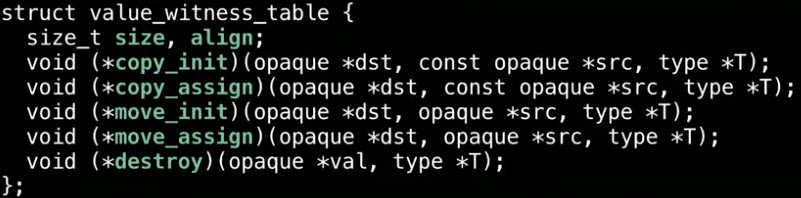
\includegraphics[width=0.7\textwidth]{/home/yukio/Diary/projs/fpcourse/fp-2024/docs/figs/swift-witness-table}
        \caption{Swift value witness table.}
        \label{fig:swift-witness-table}
    \end{figure}
    \begin{figure}
        \centering
        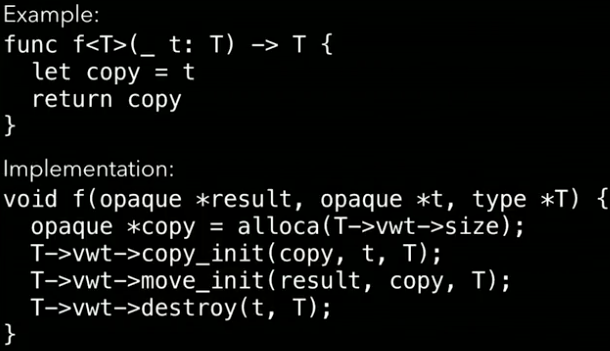
\includegraphics[width=0.6\textwidth]{/home/yukio/Diary/projs/fpcourse/fp-2024/docs/figs/swift-generated-code}
        \caption{Код полиморфной функции, порождаемый компилятором Swift.}
        \label{fig:swift-generated-code}
    \end{figure}

    \begin{itemize}
        \item[\positive] Небольшое время компиляции
        \item[\positive] Предсказуемая эффективность (не приводит к неожиданным паузам в рантайме)
        \item[\positive] Эффективная работа с value-значениями
        \item[\negative] Серьёзный константный оверхед на динамические вызовы через таблицу, эффективность очень сильно зависит от компиляторных оптимизаций
    \end{itemize}

    \subsection{Higher-kinded polymorphism}

    Haskell позволяет также абстрагироваться по типам произвольных кайндов, не только \mintinline{haskell}|Type|.
    Например, \mintinline{haskell}|f :: forall (m :: Type -> Type) a . a -> m a|.

    Говорят, что функции, возвращающие значение какого-то такого вида \texttt{m a} --- ``too polymorphic''.
    Код, использующий такие функции будет сталкиваться с серьёзнами проблемами в производительности, так как компилятор не знает конкретного типа и не может заинлайнить соответствующие вызовы \texttt{fmap}, bind, и т.д.
    Чтобы обойти эту проблему, рекомендуется пользоваться либо конкретными типами, либо воспользоваться библиотекой kan-extensions\footnote{\url{https://hackage.haskell.org/package/kan-extensions}} (см главу 13.5 в~\cite{maguire-types}).

    % todo https://bartoszmilewski.com/2017/04/17/kan-extensions/

    Далеко не во всех языках есть полиморфизм высшего ранга, но иногда он нужен.
    Например, если мы хотим объявить абстрактный тип \mintinline{haskell}|Monad|.
    Заметим, что тип кайнда \mintinline{haskell}|Type -> Type|~--- это функция на типах, принимающая один тип, и возвращающая другой.
    Соответственно, функция, абстрагированная по такому типу~--- функция высшего порядка, в некотором смысле.
    Но мы уже знаем технику избавления от них --- дефункцинализация~\cite{defunctionalization-slides}.
    Рассмотрим пример на языке Kotlin.

    Будем представлять типовую аппликацию в виде отдельного типа \mintinline{kotlin}|Apply<Sym, T>|.
    Установим, к примеру, изоморфизм между \mintinline{kotlin}|List<T>| и \mintinline{kotlin}|Apply<ListSym, T>|:
    \begin{minted}{kotlin}
        class Apply<Sym, T>(val value: Any)
        object ListSym

        fun <T> List<T>.to(): Apply<ListSym, T> = Apply(this)
        fun <T> Apply<ListSym, T>.from(): List<T> = this.value as List<T>
    \end{minted}

    Теперь мы можем объявить интерфейс монад и задать реализацию для списка с помощью синглтона:
    \begin{minted}{kotlin}
        interface Monad<M> {
            fun <T> pure(x: T): Apply<M, T>
            infix fun <T, R> Apply<M, T>.bind(k: (T) -> Apply<M, R>): Apply<M, R>
        }

        object ListMonad : Monad<ListSym> {
            override fun <T> pure(x: T): Apply<ListSym, T> = listOf(x).to()
            override fun <T, R> Apply<ListSym, T>.
                    bind(k: (T) -> Apply<ListSym, R>): Apply<ListSym, R> =
                this.from().flatMap { k(it).from() }.to()
        }
    \end{minted}

    И наконец мы можем писать функции над произвольными монадами:
    \begin{minted}{haskell}
        fun <M> Monad<M>.go(x: Apply<M, Int>): Apply<M, Int> =
            x bind { pure(it + 1) } bind { pure(it + 2) }

        fun test(xs: List<Int>): List<Int> = ListMonad.go(xs.to()).from()
    \end{minted}

    % todo можно без Any обойтись

    Не лишним будет отметить, что результирующий код выглядит несколько чудовищно.
    Скорее всего, использование этой техники не окупает себя и нужно выбирать другой стиль программирования.
    Однако иметь этот инструмент в ящике не будет лишним.

    \subsection{Полиморфизм по конвенции вызова (levity polymorphism)} \label{subsec:levity-polymorphism}

    Как мы уже обсуждали выше~\ref{subsubsec:type-erasure}, параметрический полиморфизм в Haskell реализуется следующим образом: все значения хранятся в куче и передаются в полиморфные функции по указателю.
    Однако, если для вычислительного кода важна производительность, такой подход не годится ввиду большой нагрузки на подсистему управления памятью и множества индирекций.
    Поэтому Haskell позволяет также писать код с использованием unboxed значений.
    А если код не полагается на конкретную конвенцию вызова, его можно по ней абстрагировать, и писать один код для boxed и unboxed значений~\cite{eisenberg2017levity}.

    \begin{figure}[h]
        \centering
        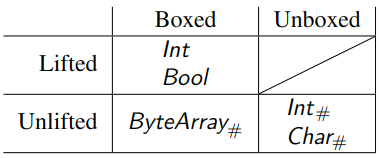
\includegraphics[width=0.5\textwidth]{/home/yukio/Diary/projs/fpcourse/fp-2024/docs/figs/haskell-value-kinds}
        \caption{Виды значений в Haskell с примерами~\cite{eisenberg2017levity}.}
        \label{fig:haskell-value-kinds}
    \end{figure}

    На рисунке~\ref{fig:haskell-value-kinds} можно увидеть классификацию значений в Haskell с примерами типов.
    \vocab{Unboxed типы} --- их значения удерживаются и передаются по значению.
    \vocab{Boxed}, соответственно, наоборот, передаются по указателю и хранятся в куче.
    Обычный \mintinline{haskell}|Int| является просто декларацией следующего вида, где \mintinline{haskell}|I#| --- это обычный конструктор, содержащий unboxed значение.
    \begin{minted}{haskell}
        data Int = I# Int#
    \end{minted}

    % todo levity

    \# в именах типов и функций --- это конвенция, показывающая, что где-то рядом происходит работа с unlifted значениями\footnote{Нужно подключить расширение MagicHash, чтобы пользоваться \# в идентификаторах.}.

    % todo \chapter*{Valhalla - Where Are We?}

    % todo data femilies for representation polymorphism

    % todo data kinds

    %todo

    % todo nim
    % todo first-class polymorphism & quick look & impredicativity


    \section{Специальный полиморфизм} \label{sec:ad-hoc}

    % todo constraints and decidability

    % todo https://chrisdone.com/posts/haskell-constraint-trick/

    % todo existential types, different vtable implementations, value types support
    % todo scala type classes
    % todo type inhabitation, system FC, Symon's talk
    % todo доклад SPJ
    % todo open unions, data a la carte
    % todo roles and coertions
    % todo typeable & reflection
    % todo reflecrtion https://www.tweag.io/blog/2017-12-21-reflection-tutorial/
    % todo How to make ad-hoc polymorphism less ad-hoc

    % todo C. V. Hall, K. Hammond, S. L. Peyton Jones, and P. L. Wadler. Type classes in haskell

    % todo S. Peyton Jones, S. Weirich, R. A. Eisenberg, and D. Vytiniotis. A reflection on types. In A list of successes that can change the world,

    % todo functional dependencies & associated types

    % todo https://downloads.haskell.org/~ghc/9.0.1/docs/html/users_guide/exts/constraints.html

    % todo


    \section{Продолжения (continuations)} \label{sec:continuations}

    % todo

    % todo связь с монадами

    % todo монада Cont

    % todo delimited continuations

    % todo sicp

    % todo raynolds The Discoveries of Continuations

    % todo correspondence to negation in intuitionistic logic?

    % todo CPS correspond to double negation in logic reynolds1998definitional

    % todo defuctionalized continuations, pepers from gibbons talk

    % todo difference lists

    % todo he Essence of Cornpiling with Continuations

    \cite{reynolds1972definitional, reynolds1998definitional, defunctionalization-slides}

    % todo jeremy gibbons papers, review the talk

    % todo delimited via undelimited and mutable cell

    \section{Интерпретаторы зазеркалья} \label{sec:wonder-interpreters}

    % todo isomorphism proof

    % todo теоретические основы

    % todo church encoding

    % todo Tagless-final интерпретаторы

    % todo codata, pattern-matching
    % todo custom patterns

    % todo fusion и дефорестация
    % todo Oleg about fusion and streams
    % todo fused effects

    % todo наверное после континуэйшенов

    % todo


    \section{Метапрограммирование и специализация}

    % todo split intro several topics

    % todo specilization, deforestation, metaprogramming
    % todo staged programming
    % todo modal types for staged programming
    % todo type roles

    % todo streams and fusion
    % todo CPS

    % todo staged computations and modal types
    % todo Haskell papers about fusion

    % todo fist class specialization to beat type families

    % todo generics and Gibbons paper about abstractions
    % todo SOP & variadics

    % todo ghc inlining paper

    % todo https://ora.ox.ac.uk/objects/uuid:cd041aa0-8d69-4f18-bce2-6d75244b69b9/files/m7fd9779b27fcb70ae734e66bcd3ee79f

%    \subsection{Template Haskell}
%
%    % todo порядок на коде для поддержания реификации
%
%    % todo
%
%    \subsection{Рефлексия и реификация}
%
%    % TODO
%
%    \subsection{Zig-generics}
%
%    % todo
%
%    \subsection{GHC.Generics}
%
%    % todo
%
%    \subsection{Uniplate}
%
%    % todo


    \section{Дополнительные главы монад}

    % todo оригинальная статья

    % todo monadic reflection
    % todo monadic reflection & direct style (lib from scala)

    % todo free monads, freer monads

    % todo монады не композируются, но фримонады - композируются

    % todo semantic domains have monad structure

    % todo https://github.com/lampepfl/monadic-reflection/blob/main/TUTORIAL.md

    % todo C# expression trees
    % todo F# что-то про монады и forM

    % todo


    \section{Хендлеры эффектов} \label{sec:effect-handlers}

    % todo алгебраические эффекты
    % todo связь с delimited continuations
    % todo стратегии компиляции, связь с codata
    % todo эффекты высших порядков
    % todo full vs shallow embeddings
    % todo abstracting definitional interpreters & github semantics
    % todo fused effects and CPS

    % todo expression problem

    % todo compare open type families & extensible interpreters

    % todo \textit{multimethods}

    Languages with \textit{multimethods}, like Common Lisp’s CLOS, Dylan, and Julia do support adding both new types and operations  easily.
    What they typically sacrifice is either static type checking, or separate compilation.


    % todo


    \section{Системы эффектов}

    % todo


    \section{Корутины}

    % todo structured concurrency

    % todo


    \section{Компилятор GHC и runtime}

    % todo


    \section{Оптика}

    % todo http://www.timphilipwilliams.com/posts/2019-07-25-minecraft.html

    % todo profunctor optics
    % todo van laarhoven CPS optics

    % todo


    % todo куда-нибудь запихнуть algebra driven design, quick check и доклад про проперти-тесты
    % todo expression problem somewhere
    % todo где-то должно быть содержание книжки про типы Sandy Maguire, data families
    % todo Perhaps Not The Answer You Were Expecting But You Asked For It
    % todo link to SICP

    % todo сказать где-нибудь про вариантность и изоморфизм

    % todo вставить куда-нибудь ссылку на F for Functor

    % todo зависимые типы в Haskell

    % todo где-то нужно про систему кайндов, константы, полиморфизм... Походу Haskell types 101.

    % todo рассовать упражнений по конспекту


    \begin{center}
        \vspace{2em}
        \textit{\LARGE To be continued...}
        \vspace{2em}
    \end{center}


    % todo что-то сделать с порядком
    \newpage
    \bibliography{bib}

\end{document}
